% ============================================================================
% Parte 03 — Stewart, Precálculo 7.ª ed., §2.3
% "Obtener información a partir de la gráfica de una función" (pp. 170–182).
%
% Ejercicios elegidos (15) y página del libro:
%   Ej.  1 (p. 178) — Conceptos: valores de la función y cambio neto desde la gráfica
%   Ej.  5 (p. 178) — Conceptos: f(x)=0 y f(x)>=0 desde la gráfica
%   Ej.  7 (p. 179) — Valores de una función (gráfica de h)
%   Ej.  9 (p. 179) — Resolver gráficamente ecuaciones y desigualdades (f y g dadas)
%   Ej. 11 (p. 179) — Dominio y rango de una gráfica: f(x)=2x+3
%   Ej. 15 (p. 179) — Dominio y rango de una gráfica: f(x)=x^2-1, -3<=x<=3
%   Ej. 21 (p. 179) — Dominio y rango de una gráfica: f(x)=sqrt(16-x^2)
%   Ej. 23 (p. 180) — Resolver gráficamente: x-2=4-x y x-2>4-x
%   Ej. 25 (p. 180) — Resolver gráficamente: x^2=2-x y x^2<=2-x
%   Ej. 31 (p. 180) — Creciente y decreciente (gráfica dada)
%   Ej. 33 (p. 180) — Creciente y decreciente (gráfica poligonal dada)
%   Ej. 43 (p. 180) — Valores de máximo y mínimo local (gráfica dada)
%   Ej. 45 (p. 180) — Valores de máximo y mínimo local (gráfica dada)
%   Ej. 55 (pp. 180–181) — Aplicación: consumo de energía eléctrica
%   Ej. 57 (p. 181) — Aplicación: función de peso
%
% Figuras extraídas del PDF del libro (pdftoppm -r 200 + recorte):
%   fig_p03_01.png (p. 178, sirve para los Ej. 1 y 5), fig_p03_07.png,
%   fig_p03_09.png, fig_p03_31.png, fig_p03_33.png, fig_p03_43.png,
%   fig_p03_45.png, fig_p03_55.png, fig_p03_57.png.
% Las gráficas de los Ej. 11, 15, 21, 23 y 25 las trazamos con pgfplots
% porque el libro no las da: hay que dibujarlas.
% ============================================================================
\documentclass[11pt]{article}
\usepackage[utf8]{inputenc}
\usepackage[spanish]{babel}
\usepackage[margin=2.3cm]{geometry}
\usepackage{amsmath,amssymb}
\usepackage{enumitem}
\usepackage{tcolorbox}
\tcbuselibrary{skins,breakable}
\usepackage{pgfplots}
\pgfplotsset{compat=1.18}
\usepackage{tikz}
\usepackage{graphicx}
\usepackage{array}
\usepackage[hidelinks]{hyperref}

% Notación española opcional (descomenta si quieres \sen en lugar de \sin)
% \DeclareMathOperator{\sen}{sen}
% \DeclareMathOperator{\tg}{tg}
% \DeclareMathOperator{\ctg}{ctg}

\newtcolorbox{sol}{colback=blue!5,colframe=blue!50!black,title=Solución paso a paso,breakable}
\newtcolorbox{teo}{colback=orange!8,colframe=orange!70!black,title=Teoría,breakable}
\newtcolorbox{nota}{colback=green!5,colframe=green!50!black,title=Idea clave,breakable}
\newtcolorbox{tip}{colback=yellow!10,colframe=yellow!60!black,title=Consejo,breakable}
\newtcolorbox{resp}{colback=red!5,colframe=red!50!black,title=Respuesta,breakable}
\newtcolorbox{reg}{colback=red!5,colframe=red!60!black,title=Regla,breakable}
\newtcolorbox{paso}[1]{colback=gray!5,colframe=gray!50!black,title={#1},breakable}

\graphicspath{{../images/}{images/}}
\newcommand{\sen}{\operatorname{sen}}

% babel spanish activa < y > y rompe TikZ/pgfplots (->, >=stealth)
\AtBeginDocument{\shorthandoff{<>}}

\begin{document}
\shorthandoff{<>}  % babel-spanish hace activos < y >; tikz/pgfplots los necesitan literales

\section*{Parte 03 — Obtener información a partir de la gráfica de una función (Stewart §2.3, pp. 170--182)}

\begin{teo}
\textbf{Método de la sección 2.3.} Todo se lee de la gráfica; no se deriva nada.
\begin{enumerate}[leftmargin=*]
\item \textbf{Valor de la función.} $f(a)$ es la \emph{altura} de la gráfica sobre el eje $x$ en $x=a$. Altura arriba del eje $\Rightarrow$ valor positivo; abajo $\Rightarrow$ negativo.
\item \textbf{Dominio y rango.} El dominio es la proyección de la gráfica sobre el eje $x$; el rango es su proyección sobre el eje $y$. Se leen como intervalos, con extremos incluidos si el punto está marcado con círculo relleno.
\item \textbf{Ecuaciones y desigualdades.} Las soluciones de $f(x)=g(x)$ son las abscisas de los puntos donde las gráficas se cruzan; las de $f(x)<g(x)$ son los $x$ donde la gráfica de $g$ está \emph{más alta} que la de $f$. Caso particular: $f(x)=0$ son las intersecciones con el eje $x$, y $f(x)\ge 0$ son los $x$ donde la gráfica está sobre o encima del eje.
\item \textbf{Crecimiento.} $f$ es creciente en un intervalo $I$ si $f(x_1)<f(x_2)$ siempre que $x_1<x_2$ en $I$; decreciente si $f(x_1)>f(x_2)$. En la gráfica: sube de izquierda a derecha $\Rightarrow$ creciente; baja $\Rightarrow$ decreciente. Por convención se reportan intervalos \emph{abiertos}.
\item \textbf{Máximos y mínimos locales.} $f(a)$ es máximo local si $f(a)\ge f(x)$ para $x$ cercana a $a$ (el punto es el más alto de su vecindad); mínimo local si $f(a)\le f(x)$. Se ubican en los picos y valles de la gráfica, justo donde el crecimiento cambia de sentido.
\item \textbf{Cambio neto.} El cambio neto de $f$ cuando la entrada pasa de $a$ a $b$ es $f(b)-f(a)$: se restan las dos alturas leídas en la gráfica.
\end{enumerate}
\end{teo}

\begin{tip}
Lo que se repite en toda la sección:
\begin{itemize}[leftmargin=*]
\item \textbf{Altura $=$ valor:} $f(a)=$ ordenada del punto de la gráfica de abscisa $a$.
\item \textbf{Cambio neto:} $f(b)-f(a)$ (no hay que dividir; eso sería razón de cambio).
\item \textbf{Máximo/mínimo local es un \emph{valor} de $y$}, y ocurre \emph{en} un valor de $x$. Se piden ambos por separado.
\item \textbf{Un extremo del dominio nunca es máximo ni mínimo local}, porque la definición exige un intervalo abierto alrededor de $a$.
\item \textbf{Para resolver $A(x)=B(x)$ gráficamente:} definí $f(x)=A(x)$ y $g(x)=B(x)$, trazá ambas y leé las abscisas de los cruces.
\end{itemize}
\end{tip}

% ===========================================================================
\subsection*{Ejercicio 1 — Valores de la función y cambio neto desde la gráfica}

\begin{quote}
\textbf{1--5 $\blacksquare$}\quad La función $f$ que se muestra a continuación se define mediante una expresión polinomial de grado 4. Utilice la gráfica para resolver los ejercicios.

\begin{center}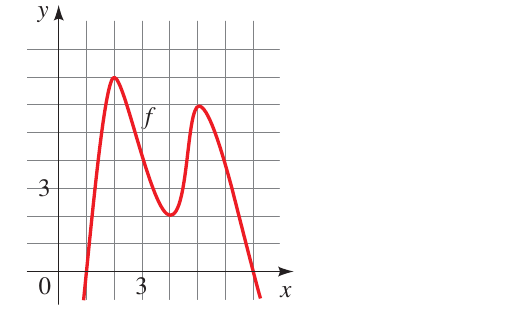
\includegraphics[width=0.42\textwidth]{fig_p03_01.png}\end{center}

\textbf{1.} Para determinar el valor de una función $f(a)$ a partir de la gráfica de $f$, encontramos la altura de la gráfica arriba del eje $x$ en $x=$ \rule{1.2cm}{0.4pt}. De la gráfica de $f$ vemos que $f(3)=$ \rule{1.2cm}{0.4pt} y $f(1)=$ \rule{0.8cm}{0.4pt}. El cambio neto en $f$ entre $x=1$ y $x=3$ es $f(\rule{0.6cm}{0.4pt})-f(\rule{0.6cm}{0.4pt})=$ \rule{0.8cm}{0.4pt}.
\end{quote}

\begin{paso}{Paso 1 --- Completar la regla de lectura}
\textbf{Qué hago:} el espacio en blanco de la primera frase se llena con $a$.

\textbf{¿De dónde sale?} De la propia frase: se busca el valor $f(a)$.

\textbf{¿Por qué?} La altura de la gráfica sobre el eje $x$ \emph{es} el valor de la función, evaluada en la abscisa correspondiente.
\end{paso}

\begin{paso}{Paso 2 --- Leer $f(3)$ y $f(1)$}
\textbf{Qué hago:} subo por la vertical $x=3$ hasta la curva y leo la altura; repito en $x=1$.

\textbf{¿De dónde sale?} De la cuadrícula de la figura: en $x=3$ la curva está en la cuarta línea horizontal; en $x=1$ la curva toca el eje $x$.

\textbf{¿Por qué?} Altura de la gráfica $=$ valor de la función (regla de lectura del paso anterior).
\[
f(3)=4, \qquad f(1)=0.
\]
\end{paso}

\begin{paso}{Paso 3 --- Calcular el cambio neto}
\textbf{Qué hago:} aplico la fórmula del cambio neto $f(b)-f(a)$ con $a=1$ y $b=3$.

\textbf{¿De dónde sale?} Los valores $4$ y $0$ vienen del paso 2; los extremos $1$ y $3$, del enunciado.

\textbf{¿Por qué?} El cambio neto se define como la diferencia entre el valor final y el inicial de la función.
\[
f(3)-f(1)=4-0=4.
\]
\end{paso}

\begin{resp}
$x=a$; \; $f(3)=4$ y $f(1)=0$; \; el cambio neto es $f(3)-f(1)=4$.
\end{resp}

% ===========================================================================
\subsection*{Ejercicio 5 — Resolver $f(x)=0$ y $f(x)\ge 0$ desde la gráfica}

\begin{quote}
\textbf{5.} Las soluciones de la ecuación $f(x)=0$ son las intersecciones \rule{1cm}{0.4pt} de la gráfica de $f$. La solución de la desigualdad $f(x)\ge 0$ es el conjunto de valores $x$ para los que la gráfica de $f$ está en el eje o sobre el eje \rule{0.8cm}{0.4pt}. De la gráfica de $f$ encontramos que las soluciones de la ecuación $f(x)=0$ son $x=$ \rule{0.8cm}{0.4pt} y $x=$ \rule{0.8cm}{0.4pt}, y la solución de la desigualdad $f(x)\ge 0$ es \rule{2.2cm}{0.4pt}.
\end{quote}

\begin{paso}{Paso 1 --- Identificar qué significa $f(x)=0$ en la gráfica}
\textbf{Qué hago:} traduzco $f(x)=0$ como ``altura cero'', es decir, intersecciones \emph{con el eje $x$}.

\textbf{¿De dónde sale?} De la regla altura $=$ valor: valor $0$ equivale a estar sobre el eje $x$.

\textbf{¿Por qué?} Los puntos del eje $x$ son exactamente los de ordenada $0$.
\end{paso}

\begin{paso}{Paso 2 --- Leer las intersecciones}
\textbf{Qué hago:} localizo dónde la curva corta el eje horizontal.

\textbf{¿De dónde sale?} De la figura: la curva cruza el eje en la primera y en la séptima línea vertical.

\textbf{¿Por qué?} Cada cruce con el eje $x$ es una solución de $f(x)=0$.
\[
x=1 \qquad\text{y}\qquad x=7.
\]
\end{paso}

\begin{paso}{Paso 3 --- Resolver la desigualdad}
\textbf{Qué hago:} tomo los $x$ donde la gráfica está sobre o encima del eje $x$.

\textbf{¿De dónde sale?} Entre $x=1$ y $x=7$ la curva está por encima del eje; fuera de ese tramo cae por debajo.

\textbf{¿Por qué?} $f(x)\ge 0$ significa altura no negativa, y los extremos se incluyen porque la desigualdad no es estricta.
\[
[\,1,\,7\,].
\]
\end{paso}

\begin{resp}
Intersecciones \textbf{con el eje $x$}; la gráfica debe estar sobre o encima del eje \textbf{$x$}; las soluciones de $f(x)=0$ son $x=1$ y $x=7$; la solución de $f(x)\ge 0$ es $[1,7]$.
\end{resp}

% ===========================================================================
\subsection*{Ejercicio 7 — Valores de una función a partir de su gráfica}

\begin{quote}
\textbf{7. Valores de una función}\quad Se da la gráfica de una función $h$.
\begin{enumerate}[label=\emph{\alph*})]
\item Encuentre $h(-2)$, $h(0)$, $h(2)$ y $h(3)$.
\item Encuentre el dominio y rango de $h$.
\item Encuentre los valores de $x$ para los cuales $h(x)=3$.
\item Encuentre los valores de $x$ para los cuales $h(x)\le 3$.
\item Encuentre el cambio neto de $h$ entre $x=-3$ y $x=3$.
\end{enumerate}

\begin{center}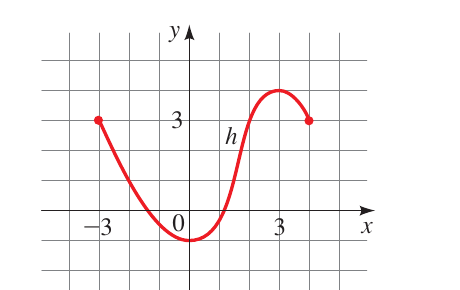
\includegraphics[width=0.5\textwidth]{fig_p03_07.png}\end{center}
\end{quote}

\begin{paso}{Paso 1 --- Leer las cuatro alturas del inciso \emph{a})}
\textbf{Qué hago:} sobre cada abscisa pedida subo hasta la curva y leo la ordenada en la cuadrícula.

\textbf{¿De dónde sale?} De la figura: en $x=-2$ la curva está una unidad arriba del eje; en $x=0$ está una unidad abajo (es el punto más bajo); en $x=2$ está en $y=3$; en $x=3$ está en el pico, $y=4$.

\textbf{¿Por qué?} Altura de la gráfica $=$ valor de la función.
\[
h(-2)=1,\quad h(0)=-1,\quad h(2)=3,\quad h(3)=4.
\]
\end{paso}

\begin{paso}{Paso 2 --- Dominio y rango por proyección}
\textbf{Qué hago:} proyecto la gráfica sobre el eje $x$ y sobre el eje $y$.

\textbf{¿De dónde sale?} La curva empieza en el punto marcado $(-3,3)$ y termina en el punto marcado $(4,3)$; su altura mínima es $-1$ (en $x=0$) y la máxima es $4$ (en $x=3$).

\textbf{¿Por qué?} El dominio son las entradas que aparecen en la gráfica y el rango las salidas; los puntos están rellenos, así que los extremos se incluyen.
\[
\text{Dominio } [-3,4], \qquad \text{Rango } [-1,4].
\]
\end{paso}

\begin{paso}{Paso 3 --- Resolver $h(x)=3$}
\textbf{Qué hago:} corto la gráfica con la recta horizontal $y=3$ y leo las abscisas de los cortes.

\textbf{¿De dónde sale?} La recta $y=3$ pasa por el extremo izquierdo $(-3,3)$, corta la rama creciente en $x=2$ y pasa por el extremo derecho $(4,3)$.

\textbf{¿Por qué?} $h(x)=3$ pide los puntos de la gráfica cuya altura vale exactamente $3$.
\[
x=-3,\quad x=2,\quad x=4.
\]
\end{paso}

\begin{paso}{Paso 4 --- Resolver $h(x)\le 3$}
\textbf{Qué hago:} tomo los $x$ del dominio donde la gráfica está en la recta $y=3$ o por debajo de ella.

\textbf{¿De dónde sale?} Del paso 3: la gráfica queda por debajo de $y=3$ desde $x=-3$ hasta $x=2$, y entre $x=2$ y $x=4$ está por encima, salvo en el extremo $x=4$, donde vale exactamente $3$.

\textbf{¿Por qué?} La desigualdad no estricta admite también los puntos de igualdad hallados en el paso 3.
\[
[-3,2]\;\cup\;\{4\}.
\]
\end{paso}

\begin{paso}{Paso 5 --- Cambio neto entre $x=-3$ y $x=3$}
\textbf{Qué hago:} aplico $h(b)-h(a)$ con $a=-3$ y $b=3$.

\textbf{¿De dónde sale?} $h(3)=4$ es del paso 1 y $h(-3)=3$ se lee en el punto extremo izquierdo.

\textbf{¿Por qué?} El cambio neto es la diferencia de los valores en los extremos, no un promedio.
\[
h(3)-h(-3)=4-3=1.
\]
\end{paso}

\begin{resp}
\emph{a}) $h(-2)=1$, $h(0)=-1$, $h(2)=3$, $h(3)=4$. \quad
\emph{b}) Dominio $[-3,4]$, rango $[-1,4]$. \quad
\emph{c}) $x=-3,\;2,\;4$. \quad
\emph{d}) $[-3,2]\cup\{4\}$. \quad
\emph{e}) Cambio neto $=1$.
\end{resp}

% ===========================================================================
\subsection*{Ejercicio 9 — Comparar dos funciones: ecuaciones y desigualdades gráficas}

\begin{quote}
\textbf{9. Resolver gráficamente ecuaciones y desigualdades}\quad Se dan las gráficas de las funciones $f$ y $g$.
\begin{enumerate}[label=\emph{\alph*})]
\item ¿Cuál es mayor, $f(0)$ o $g(0)$?
\item ¿Cuál es mayor, $f(-3)$ o $g(-3)$?
\item ¿Para qué valores de $x$ es $f(x)=g(x)$?
\item Encuentre los valores de $x$ para los cuales $f(x)\le g(x)$.
\item Encuentre los valores de $x$ para los cuales $f(x)>g(x)$.
\end{enumerate}

\begin{center}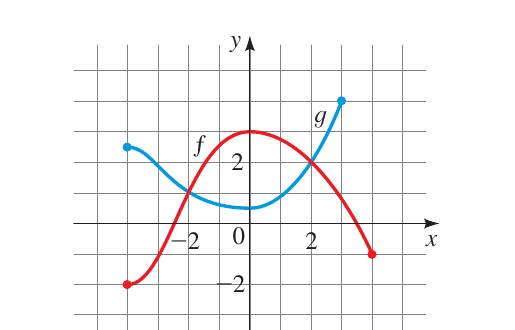
\includegraphics[width=0.52\textwidth]{fig_p03_09.png}\end{center}
\end{quote}

\begin{paso}{Paso 1 --- Comparar alturas en $x=0$ y en $x=-3$}
\textbf{Qué hago:} en cada abscisa miro cuál de las dos curvas está más arriba.

\textbf{¿De dónde sale?} En $x=0$ la curva roja ($f$) está en su punto más alto, $f(0)=3$, mientras que la azul ($g$) está en su valle, cerca de $y=0.5$. En $x=-3$ la roja está bajo el eje ($\approx-1$) y la azul está cerca de $y=2$.

\textbf{¿Por qué?} Comparar $f(a)$ con $g(a)$ es comparar alturas sobre la misma vertical $x=a$.
\[
f(0)>g(0), \qquad g(-3)>f(-3).
\]
\end{paso}

\begin{paso}{Paso 2 --- Resolver $f(x)=g(x)$}
\textbf{Qué hago:} localizo los puntos donde las dos gráficas se cruzan y leo sus abscisas.

\textbf{¿De dónde sale?} De la figura: los cruces ocurren sobre las verticales $x=-2$ y $x=2$.

\textbf{¿Por qué?} Las soluciones de $f(x)=g(x)$ son los valores de $x$ en que las dos gráficas se intersecan.
\[
x=-2 \qquad\text{y}\qquad x=2.
\]
\end{paso}

\begin{paso}{Paso 3 --- Resolver $f(x)\le g(x)$}
\textbf{Qué hago:} tomo los $x$ donde la gráfica de $g$ está más alta que la de $f$, agregando los cruces.

\textbf{¿De dónde sale?} Los cruces $x=-2$ y $x=2$ del paso 2 parten el dominio común; a la izquierda de $-2$ y a la derecha de $2$ la azul va por encima. La gráfica de $g$ termina en $x=3$ y ambas empiezan en $x=-4$.

\textbf{¿Por qué?} $f(x)\le g(x)$ describe los $x$ donde $g$ está encima de $f$ o a la misma altura; solo tiene sentido donde ambas están definidas.
\[
[-4,-2]\;\cup\;[2,3].
\]
\end{paso}

\begin{paso}{Paso 4 --- Resolver $f(x)>g(x)$}
\textbf{Qué hago:} tomo el tramo restante, sin incluir los cruces.

\textbf{¿De dónde sale?} Entre $x=-2$ y $x=2$ la roja va por encima de la azul (paso 3).

\textbf{¿Por qué?} La desigualdad estricta excluye los puntos donde las gráficas se tocan.
\[
(-2,2).
\]
\end{paso}

\begin{resp}
\emph{a}) $f(0)$ es mayor. \quad \emph{b}) $g(-3)$ es mayor. \quad \emph{c}) $x=-2$ y $x=2$. \quad
\emph{d}) $[-4,-2]\cup[2,3]$. \quad \emph{e}) $(-2,2)$.
\end{resp}

% ===========================================================================
\subsection*{Ejercicio 11 — Dominio y rango a partir de la gráfica: $f(x)=2x+3$}

\begin{quote}
\textbf{11--16 $\blacksquare$ Dominio y rango de una gráfica}\quad Se da una función $f$. \emph{a}) trace una gráfica de $f$. \emph{b}) Utilice una gráfica para encontrar el dominio y el rango de $f$.

\textbf{11.} $f(x)=2x+3$
\end{quote}

\begin{paso}{Paso 1 --- Trazar la gráfica}
\textbf{Qué hago:} reconozco una función lineal $f(x)=ax+b$ con $a=2$, $b=3$, y la trazo con dos puntos: $(0,3)$ y $(1,5)$.

\textbf{¿De dónde sale?} De la fórmula del enunciado, evaluada en $x=0$ y $x=1$.

\textbf{¿Por qué?} La gráfica de una función lineal es una recta, y dos puntos la determinan.
\begin{center}
\begin{tikzpicture}
\begin{axis}[width=8cm,height=5.6cm,axis lines=middle,xlabel={$x$},ylabel={$y$},
  xmin=-4.5,xmax=3.5,ymin=-6,ymax=9,grid=both,grid style={gray!25},
  xtick={-4,-2,0,2},ytick={-4,-2,2,4,6,8},samples=2]
\addplot[very thick,red,domain=-4.2:3.2]{2*x+3};
\addplot[only marks,mark=*,red] coordinates {(0,3) (1,5)};
\end{axis}
\end{tikzpicture}
\end{center}
\end{paso}

\begin{paso}{Paso 2 --- Leer dominio y rango por proyección}
\textbf{Qué hago:} proyecto la recta sobre cada eje.

\textbf{¿De dónde sale?} De la gráfica del paso 1: la recta no es horizontal y se extiende indefinidamente en ambos sentidos.

\textbf{¿Por qué?} El dominio es la proyección sobre el eje $x$ y el rango la proyección sobre el eje $y$; una recta de pendiente $2\ne 0$ cubre todos los valores de ambos ejes.
\[
\text{Dominio } (-\infty,\infty), \qquad \text{Rango } (-\infty,\infty).
\]
\end{paso}

\begin{resp}
La gráfica es la recta de pendiente $2$ e intersección $y$ igual a $3$; dominio $\mathbb{R}=(-\infty,\infty)$ y rango $\mathbb{R}=(-\infty,\infty)$.
\end{resp}

% ===========================================================================
\subsection*{Ejercicio 15 — Dominio y rango a partir de la gráfica: parábola restringida}

\begin{quote}
\textbf{15.} $f(x)=x^2-1$, $-3\le x\le 3$
\end{quote}

\begin{paso}{Paso 1 --- Trazar el arco de parábola}
\textbf{Qué hago:} tabulo $f$ en los enteros del intervalo dado y uno los puntos con la parábola $y=x^2-1$.

\textbf{¿De dónde sale?} De la fórmula: $f(0)=-1$, $f(\pm1)=0$, $f(\pm2)=3$, $f(\pm3)=8$.

\textbf{¿Por qué?} $y=x^2-1$ es la parábola $y=x^2$ trasladada $1$ unidad hacia abajo; el enunciado la corta en $-3\le x\le 3$.
\begin{center}
\begin{tikzpicture}
\begin{axis}[width=8cm,height=5.8cm,axis lines=middle,xlabel={$x$},ylabel={$y$},
  xmin=-4.2,xmax=4.2,ymin=-2.5,ymax=9.5,grid=both,grid style={gray!25},
  xtick={-3,-2,-1,1,2,3},ytick={-1,2,4,6,8},samples=100]
\addplot[very thick,red,domain=-3:3]{x^2-1};
\addplot[only marks,mark=*,red] coordinates {(-3,8) (3,8) (0,-1)};
\end{axis}
\end{tikzpicture}
\end{center}
\end{paso}

\begin{paso}{Paso 2 --- Leer dominio y rango}
\textbf{Qué hago:} proyecto el arco dibujado sobre los dos ejes.

\textbf{¿De dónde sale?} El dominio lo impone el enunciado, $-3\le x\le 3$; la altura mínima es $f(0)=-1$ (vértice) y la máxima es $f(\pm3)=8$ (extremos), del paso 1.

\textbf{¿Por qué?} El rango de una función continua sobre un intervalo cerrado va del valor más bajo al más alto que efectivamente alcanza; ambos extremos se alcanzan, así que el intervalo es cerrado.
\[
\text{Dominio } [-3,3], \qquad \text{Rango } [-1,8].
\]
\end{paso}

\begin{resp}
Dominio $[-3,3]$; rango $[-1,8]$.
\end{resp}

% ===========================================================================
\subsection*{Ejercicio 21 — Dominio y rango a partir de la gráfica: $f(x)=\sqrt{16-x^2}$}

\begin{quote}
\textbf{17--22 $\blacksquare$ Determinación gráfica de dominio y rango}\quad Se da una función $f$. \emph{a}) Use una calculadora graficadora para trazar la gráfica de $f$. \emph{b}) Encuentre el dominio y el rango de $f$ a partir de la gráfica.

\textbf{21.} $f(x)=\sqrt{16-x^2}$
\end{quote}

\begin{paso}{Paso 1 --- Restricción del radicando}
\textbf{Qué hago:} exijo $16-x^2\ge 0$ para que la raíz cuadrada esté definida en $\mathbb{R}$.

\textbf{¿De dónde sale?} Del enunciado: el radicando de $f$ es $16-x^2$.

\textbf{¿Por qué?} La raíz de índice par solo está definida para argumentos no negativos en los reales.
\[
16-x^2\ge 0 \;\Longleftrightarrow\; x^2\le 16 \;\Longleftrightarrow\; -4\le x\le 4.
\]
\end{paso}

\begin{paso}{Paso 2 --- Reconocer la curva}
\textbf{Qué hago:} elevo al cuadrado para identificar la forma: $y=\sqrt{16-x^2}$ con $y\ge0$ equivale a $x^2+y^2=16$ con $y\ge0$.

\textbf{¿De dónde sale?} De la fórmula del enunciado, elevando ambos lados al cuadrado.

\textbf{¿Por qué?} $x^2+y^2=16$ es la circunferencia de centro el origen y radio $4$; la condición $y\ge0$ deja solo la semicircunferencia superior.
\begin{center}
\begin{tikzpicture}
\begin{axis}[width=8.4cm,height=5cm,axis lines=middle,xlabel={$x$},ylabel={$y$},
  xmin=-5.4,xmax=5.4,ymin=-1,ymax=5.2,grid=both,grid style={gray!25},
  xtick={-4,-2,2,4},ytick={2,4},samples=200]
\addplot[very thick,red,domain=-4:4]{sqrt(16-x^2)};
\addplot[only marks,mark=*,red] coordinates {(-4,0) (4,0) (0,4)};
\end{axis}
\end{tikzpicture}
\end{center}
\end{paso}

\begin{paso}{Paso 3 --- Leer dominio y rango}
\textbf{Qué hago:} proyecto la semicircunferencia sobre los dos ejes.

\textbf{¿De dónde sale?} El dominio $[-4,4]$ del paso 1; la altura va de $0$ (en $x=\pm4$) hasta $4$ (en $x=0$), del paso 2.

\textbf{¿Por qué?} Dominio y rango son las proyecciones de la gráfica sobre el eje $x$ y el eje $y$, respectivamente.
\[
\text{Dominio } [-4,4], \qquad \text{Rango } [0,4].
\]
\end{paso}

\begin{resp}
La gráfica es la semicircunferencia superior de centro el origen y radio $4$; dominio $[-4,4]$ y rango $[0,4]$.
\end{resp}

% ===========================================================================
\subsection*{Ejercicio 23 — Resolver gráficamente una ecuación y una desigualdad lineales}

\begin{quote}
\textbf{23--26 $\blacksquare$ Resolver gráficamente ecuaciones y desigualdades}\quad Resuelva en forma gráfica la ecuación o desigualdad dadas.

\textbf{23.} \emph{a}) $x-2=4-x$ \hfill \emph{b}) $x-2>4-x$
\end{quote}

\begin{paso}{Paso 1 --- Definir las dos funciones y trazarlas}
\textbf{Qué hago:} llamo $f(x)=x-2$ al lado izquierdo y $g(x)=4-x$ al lado derecho, y trazo ambas rectas en los mismos ejes.

\textbf{¿De dónde sale?} Directamente del enunciado, un lado de la igualdad para cada función.

\textbf{¿Por qué?} El método gráfico de la sección convierte la ecuación en la comparación $f(x)=g(x)$, cuyas soluciones son los cruces de las gráficas.
\begin{center}
\begin{tikzpicture}
\begin{axis}[width=8.6cm,height=5.4cm,axis lines=middle,xlabel={$x$},ylabel={$y$},
  xmin=-1.5,xmax=6.5,ymin=-3.5,ymax=5.5,grid=both,grid style={gray!25},
  xtick={1,2,3,4,5,6},ytick={-2,2,4},samples=2,legend style={at={(0.02,0.98)},anchor=north west,font=\small}]
\addplot[very thick,red,domain=-1.2:6.2]{x-2}; \addlegendentry{$f(x)=x-2$}
\addplot[very thick,blue,domain=-1.2:6.2]{4-x}; \addlegendentry{$g(x)=4-x$}
\addplot[only marks,mark=*,black] coordinates {(3,1)};
\end{axis}
\end{tikzpicture}
\end{center}
\end{paso}

\begin{paso}{Paso 2 --- Leer el cruce}
\textbf{Qué hago:} leo la abscisa del único punto de intersección.

\textbf{¿De dónde sale?} De la gráfica: las dos rectas se cortan en $(3,1)$.

\textbf{¿Por qué?} En el cruce las dos alturas coinciden, o sea $f(x)=g(x)$; hay uno solo porque las pendientes $1$ y $-1$ son distintas.
\[
x=3.
\]
\end{paso}

\begin{paso}{Paso 3 --- Leer la desigualdad $f(x)>g(x)$}
\textbf{Qué hago:} tomo los $x$ donde la recta roja está \emph{más alta} que la azul.

\textbf{¿De dónde sale?} Del paso 2: a la derecha de $x=3$ la recta creciente $f$ queda por encima de la decreciente $g$.

\textbf{¿Por qué?} $f(x)>g(x)$ describe los $x$ donde la gráfica de $f$ está estrictamente por encima de la de $g$; el cruce se excluye por ser desigualdad estricta.
\[
(3,\infty).
\]
\end{paso}

\begin{resp}
\emph{a}) $x=3$. \quad \emph{b}) $(3,\infty)$, es decir $x>3$.
\end{resp}

% ===========================================================================
\subsection*{Ejercicio 25 — Resolver gráficamente una ecuación cuadrática y su desigualdad}

\begin{quote}
\textbf{25.} \emph{a}) $x^2=2-x$ \hfill \emph{b}) $x^2\le 2-x$
\end{quote}

\begin{paso}{Paso 1 --- Definir las funciones y trazarlas}
\textbf{Qué hago:} tomo $f(x)=x^2$ y $g(x)=2-x$ y las grafico juntas.

\textbf{¿De dónde sale?} Del enunciado: un lado de la igualdad para cada función.

\textbf{¿Por qué?} Las soluciones de $f(x)=g(x)$ son las abscisas de los cruces de las dos gráficas.
\begin{center}
\begin{tikzpicture}
\begin{axis}[width=8.6cm,height=5.6cm,axis lines=middle,xlabel={$x$},ylabel={$y$},
  xmin=-3.6,xmax=2.6,ymin=-1.2,ymax=6.2,grid=both,grid style={gray!25},
  xtick={-3,-2,-1,1,2},ytick={1,2,3,4,5},samples=120,
  legend style={at={(0.98,0.98)},anchor=north east,font=\small}]
\addplot[very thick,red,domain=-3.2:2.4]{x^2}; \addlegendentry{$f(x)=x^2$}
\addplot[very thick,blue,domain=-3.4:2.4]{2-x}; \addlegendentry{$g(x)=2-x$}
\addplot[only marks,mark=*,black] coordinates {(-2,4) (1,1)};
\end{axis}
\end{tikzpicture}
\end{center}
\end{paso}

\begin{paso}{Paso 2 --- Leer los cruces}
\textbf{Qué hago:} leo las abscisas de los dos puntos de intersección.

\textbf{¿De dónde sale?} De la gráfica: la parábola y la recta se cortan en $(-2,4)$ y en $(1,1)$.

\textbf{¿Por qué?} Cada cruce da una solución de $f(x)=g(x)$, es decir de $x^2=2-x$.
\[
x=-2 \qquad\text{y}\qquad x=1.
\]
\end{paso}

\begin{paso}{Paso 3 --- Verificar los dos valores}
\textbf{Qué hago:} sustituyo cada valor en la ecuación original.

\textbf{¿De dónde sale?} De los cruces del paso 2 y de la ecuación $x^2=2-x$ del enunciado.

\textbf{¿Por qué?} La lectura gráfica es aproximada; la sustitución confirma que los valores leídos son exactos.
\[
(-2)^2=4=2-(-2), \qquad 1^2=1=2-1.
\]
\end{paso}

\begin{paso}{Paso 4 --- Leer la desigualdad $f(x)\le g(x)$}
\textbf{Qué hago:} tomo los $x$ donde la parábola está por debajo de la recta o a la misma altura.

\textbf{¿De dónde sale?} De la gráfica: entre los cruces $x=-2$ y $x=1$ la recta azul va por encima de la parábola roja.

\textbf{¿Por qué?} $f(x)\le g(x)$ son los $x$ donde la gráfica de $g$ está más alta que la de $f$, incluyendo los cruces por no ser estricta.
\[
[-2,1].
\]
\end{paso}

\begin{resp}
\emph{a}) $x=-2$ y $x=1$. \quad \emph{b}) $[-2,1]$.
\end{resp}

% ===========================================================================
\subsection*{Ejercicio 31 — Intervalos de crecimiento y decrecimiento}

\begin{quote}
\textbf{31--34 $\blacksquare$ Creciente y decreciente}\quad Se da la gráfica de una función $f$. Utilice la gráfica para estimar lo siguiente. \emph{a}) El dominio y el rango de $f$. \emph{b}) Los intervalos en los que $f$ es creciente y en los que $f$ es decreciente.

\textbf{31.}
\begin{center}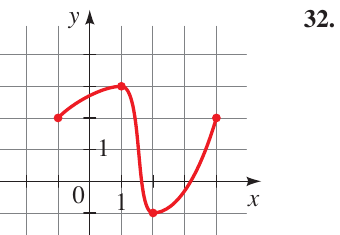
\includegraphics[width=0.45\textwidth]{fig_p03_31.png}\end{center}
\end{quote}

\begin{paso}{Paso 1 --- Dominio y rango por proyección}
\textbf{Qué hago:} proyecto la curva sobre los dos ejes.

\textbf{¿De dónde sale?} De la figura: la gráfica empieza en el punto marcado $(-1,2)$ y termina en el punto marcado $(4,2)$; su punto más alto es $(1,3)$ y el más bajo $(2,-1)$.

\textbf{¿Por qué?} Dominio y rango son las proyecciones sobre el eje $x$ y el eje $y$; los puntos rellenos incluyen los extremos.
\[
\text{Dominio } [-1,4], \qquad \text{Rango } [-1,3].
\]
\end{paso}

\begin{paso}{Paso 2 --- Localizar los cambios de sentido}
\textbf{Qué hago:} recorro la gráfica de izquierda a derecha y marco dónde deja de subir y dónde deja de bajar.

\textbf{¿De dónde sale?} De la figura: sube desde $(-1,2)$ hasta el pico $(1,3)$, baja hasta el valle $(2,-1)$, y vuelve a subir hasta $(4,2)$.

\textbf{¿Por qué?} $f$ es creciente donde la gráfica sube de izquierda a derecha y decreciente donde baja (definición de la sección).
\end{paso}

\begin{paso}{Paso 3 --- Escribir los intervalos}
\textbf{Qué hago:} traduzco los tramos del paso 2 a intervalos abiertos.

\textbf{¿De dónde sale?} De las abscisas $-1$, $1$, $2$ y $4$ halladas en el paso 2.

\textbf{¿Por qué?} Por convención los intervalos de monotonía se escriben abiertos, porque la definición compara pares de puntos dentro del intervalo.
\[
\text{Creciente en } (-1,1)\text{ y } (2,4); \qquad \text{decreciente en } (1,2).
\]
\end{paso}

\begin{resp}
\emph{a}) Dominio $[-1,4]$, rango $[-1,3]$. \quad
\emph{b}) Creciente en $(-1,1)$ y $(2,4)$; decreciente en $(1,2)$.
\end{resp}

% ===========================================================================
\subsection*{Ejercicio 33 — Crecimiento y decrecimiento en una gráfica poligonal}

\begin{quote}
\textbf{33.}
\begin{center}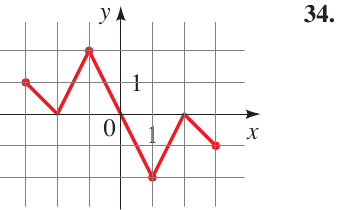
\includegraphics[width=0.45\textwidth]{fig_p03_33.png}\end{center}
\end{quote}

\begin{paso}{Paso 1 --- Leer los vértices de la poligonal}
\textbf{Qué hago:} anoto las coordenadas de los puntos donde la gráfica quiebra.

\textbf{¿De dónde sale?} De la cuadrícula de la figura, leyendo cada esquina.

\textbf{¿Por qué?} Una gráfica formada por segmentos queda determinada por sus vértices, y entre vértices consecutivos el sentido de variación no cambia.
\[
(-2,1),\;(-1,0),\;(0,2),\;(2,-2),\;(3,0),\;(4,-1).
\]
\end{paso}

\begin{paso}{Paso 2 --- Dominio y rango}
\textbf{Qué hago:} proyecto la poligonal sobre los dos ejes.

\textbf{¿De dónde sale?} De la lista de vértices del paso 1: la primera abscisa es $-2$ y la última $4$; la altura menor es $-2$ y la mayor $2$.

\textbf{¿Por qué?} Los valores extremos de una poligonal se alcanzan en sus vértices, así que basta mirar la lista.
\[
\text{Dominio } [-2,4], \qquad \text{Rango } [-2,2].
\]
\end{paso}

\begin{paso}{Paso 3 --- Clasificar cada segmento}
\textbf{Qué hago:} comparo las alturas de los extremos de cada segmento consecutivo.

\textbf{¿De dónde sale?} De los vértices del paso 1.

\textbf{¿Por qué?} Un segmento sube si la ordenada final supera a la inicial (creciente) y baja en caso contrario (decreciente).
\[
\begin{array}{ll}
1\to 0 \text{ en } [-2,-1]: \text{baja} & 0\to 2 \text{ en } [-1,0]: \text{sube}\\
2\to -2 \text{ en } [0,2]: \text{baja} & -2\to 0 \text{ en } [2,3]: \text{sube}\\
0\to -1 \text{ en } [3,4]: \text{baja} &
\end{array}
\]
\end{paso}

\begin{resp}
\emph{a}) Dominio $[-2,4]$, rango $[-2,2]$. \quad
\emph{b}) Creciente en $(-1,0)$ y $(2,3)$; decreciente en $(-2,-1)$, $(0,2)$ y $(3,4)$.
\end{resp}

% ===========================================================================
\subsection*{Ejercicio 43 — Máximos y mínimos locales leídos de la gráfica}

\begin{quote}
\textbf{43--46 $\blacksquare$ Valores de máximo y mínimo local}\quad Se da la gráfica de una función. Utilice la gráfica para calcular lo siguiente. \emph{a}) Encuentre todos los valores máximo y mínimo locales de la función y el valor de $x$ en el que ocurre cada uno. \emph{b}) Encuentre los intervalos en los que la función es creciente y en los que la función es decreciente.

\textbf{43.}
\begin{center}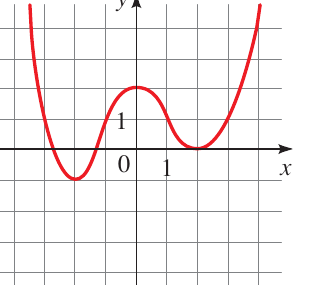
\includegraphics[width=0.4\textwidth]{fig_p03_43.png}\end{center}
\end{quote}

\begin{paso}{Paso 1 --- Ubicar picos y valles}
\textbf{Qué hago:} recorro la gráfica y marco los puntos donde cambia el sentido de variación.

\textbf{¿De dónde sale?} De la figura: hay un valle en $x=-1$, un pico en $x=1$ y otro valle en $x=3$.

\textbf{¿Por qué?} Un máximo o mínimo local ocurre exactamente donde la gráfica deja de subir y empieza a bajar, o al revés.
\end{paso}

\begin{paso}{Paso 2 --- Leer los valores en la cuadrícula}
\textbf{Qué hago:} leo la altura de cada uno de los tres puntos del paso 1.

\textbf{¿De dónde sale?} De la cuadrícula: el valle izquierdo está una unidad bajo el eje, el pico está en la segunda línea sobre el eje y el valle derecho está \emph{sobre} el eje.

\textbf{¿Por qué?} El máximo (o mínimo) local es el \emph{valor} de la función, es decir la ordenada del punto.
\[
\text{mínimo local } -1 \text{ en } x=-1;\quad
\text{máximo local } 2 \text{ en } x=1;\quad
\text{mínimo local } 0 \text{ en } x=3.
\]
\end{paso}

\begin{paso}{Paso 3 --- Intervalos de monotonía}
\textbf{Qué hago:} entre extremos consecutivos leo si la gráfica sube o baja, y agrego las ramas infinitas.

\textbf{¿De dónde sale?} De las abscisas $-1$, $1$ y $3$ del paso 1, y de que ambas ramas laterales de la gráfica se disparan hacia arriba.

\textbf{¿Por qué?} El sentido de variación solo puede cambiar en los puntos localizados en el paso 1.
\[
\text{Creciente en } (-1,1) \text{ y } (3,\infty); \qquad \text{decreciente en } (-\infty,-1) \text{ y } (1,3).
\]
\end{paso}

\begin{resp}
\emph{a}) Mínimo local $-1$ en $x=-1$; máximo local $2$ en $x=1$; mínimo local $0$ en $x=3$. \quad
\emph{b}) Creciente en $(-1,1)$ y $(3,\infty)$; decreciente en $(-\infty,-1)$ y $(1,3)$.
\end{resp}

% ===========================================================================
\subsection*{Ejercicio 45 — Cuatro extremos locales en una misma gráfica}

\begin{quote}
\textbf{45.}
\begin{center}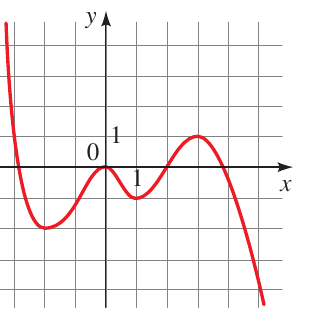
\includegraphics[width=0.4\textwidth]{fig_p03_45.png}\end{center}
\end{quote}

\begin{paso}{Paso 1 --- Ubicar los cuatro cambios de sentido}
\textbf{Qué hago:} recorro la curva de izquierda a derecha y marco cada pico y cada valle.

\textbf{¿De dónde sale?} De la figura: valle en $x=-2$, pico en $x=0$, valle en $x=1$ y pico en $x=3$.

\textbf{¿Por qué?} Los extremos locales están donde la gráfica deja de bajar y empieza a subir (mínimo) o al revés (máximo).
\end{paso}

\begin{paso}{Paso 2 --- Leer las cuatro alturas}
\textbf{Qué hago:} leo la ordenada de cada uno de esos cuatro puntos en la cuadrícula.

\textbf{¿De dónde sale?} De la figura: el valle izquierdo está dos unidades bajo el eje; el primer pico está \emph{sobre} el eje; el segundo valle, una unidad abajo; el pico derecho, una unidad arriba.

\textbf{¿Por qué?} Máximo y mínimo locales son valores de $y$, no de $x$.
\[
\begin{array}{ll}
\text{mínimo local } -2 \text{ en } x=-2, & \text{máximo local } 0 \text{ en } x=0,\\
\text{mínimo local } -1 \text{ en } x=1, & \text{máximo local } 1 \text{ en } x=3.
\end{array}
\]
\end{paso}

\begin{paso}{Paso 3 --- Intervalos de monotonía}
\textbf{Qué hago:} alterno crecimiento y decrecimiento entre extremos consecutivos, incluyendo las ramas infinitas.

\textbf{¿De dónde sale?} De las abscisas $-2$, $0$, $1$ y $3$ del paso 1; a la izquierda la gráfica baja desde arriba y a la derecha se hunde.

\textbf{¿Por qué?} Entre dos extremos locales consecutivos la función no puede cambiar de sentido.
\[
\text{Creciente en } (-2,0) \text{ y } (1,3); \qquad
\text{decreciente en } (-\infty,-2),\;(0,1) \text{ y } (3,\infty).
\]
\end{paso}

\begin{resp}
\emph{a}) Mínimos locales: $-2$ en $x=-2$ y $-1$ en $x=1$. Máximos locales: $0$ en $x=0$ y $1$ en $x=3$. \quad
\emph{b}) Creciente en $(-2,0)$ y $(1,3)$; decreciente en $(-\infty,-2)$, $(0,1)$ y $(3,\infty)$.
\end{resp}

% ===========================================================================
\subsection*{Ejercicio 55 — Aplicación: consumo de energía eléctrica}

\begin{quote}
\textbf{55. Consumo de energía eléctrica}\quad La figura muestra el consumo de energía eléctrica en San Francisco para un día de septiembre ($P$ se mide en megawatts; $t$ se mide en horas empezando a la medianoche).
\begin{enumerate}[label=\emph{\alph*})]
\item ¿Cuál fue el consumo de energía eléctrica a las 6:00 a.m.? Y cuál, a las 6:00 p.m.?
\item ¿Cuándo fue el mínimo consumo de energía eléctrica?
\item ¿Cuándo fue el máximo consumo de energía eléctrica?
\item Encuentre el cambio neto en el consumo de energía de 9:00 a.m. a 7:00 p.m.
\end{enumerate}

\begin{center}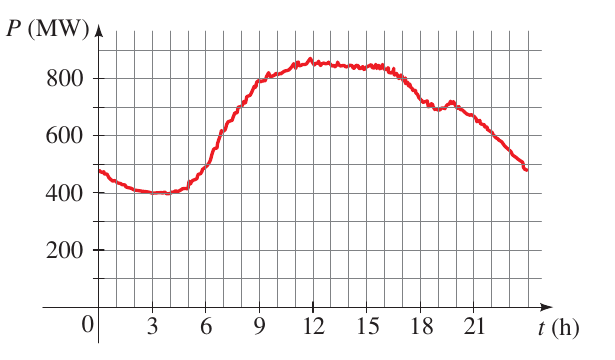
\includegraphics[width=0.72\textwidth]{fig_p03_55.png}\end{center}
\end{quote}

\begin{paso}{Paso 1 --- Traducir las horas a valores de $t$}
\textbf{Qué hago:} convierto cada hora del reloj al eje $t$, que cuenta horas desde la medianoche.

\textbf{¿De dónde sale?} Del enunciado, que fija $t=0$ a la medianoche.

\textbf{¿Por qué?} Sin esta traducción no se puede localizar la vertical correcta en la gráfica.
\[
\text{6:00 a.m.}\to t=6,\quad \text{9:00 a.m.}\to t=9,\quad \text{6:00 p.m.}\to t=18,\quad \text{7:00 p.m.}\to t=19.
\]
\end{paso}

\begin{paso}{Paso 2 --- Leer los consumos del inciso \emph{a})}
\textbf{Qué hago:} leo la altura de la curva en $t=6$ y en $t=18$.

\textbf{¿De dónde sale?} De la cuadrícula: en $t=6$ la curva está a la mitad entre las líneas de $400$ y $600$; en $t=18$ está algo por encima de la línea de $700$.

\textbf{¿Por qué?} Altura de la gráfica $=$ valor de $P$, en megawatts.
\[
P(6)\approx 500\ \text{MW}, \qquad P(18)\approx 730\ \text{MW}.
\]
\end{paso}

\begin{paso}{Paso 3 --- Mínimo y máximo del día}
\textbf{Qué hago:} busco el punto más bajo y el más alto de la curva y leo su abscisa.

\textbf{¿De dónde sale?} De la figura: el tramo más bajo, de unos $400$ MW, está entre $t=3$ y $t=4$; el pico, de unos $850$ MW, está cerca de $t=12$.

\textbf{¿Por qué?} El mínimo y el máximo del día son el punto más bajo y el más alto de la gráfica en todo el intervalo mostrado.
\[
\text{mínimo} \approx 400\ \text{MW cerca de las 4:00 a.m.};\qquad
\text{máximo} \approx 850\ \text{MW cerca del mediodía}.
\]
\end{paso}

\begin{paso}{Paso 4 --- Cambio neto de 9:00 a.m. a 7:00 p.m.}
\textbf{Qué hago:} aplico $P(19)-P(9)$ con las alturas leídas en esas dos verticales.

\textbf{¿De dónde sale?} De la gráfica: $P(9)\approx 800$ MW y $P(19)\approx 700$ MW; las horas vienen del paso 1.

\textbf{¿Por qué?} El cambio neto es la diferencia entre el valor final y el inicial; sale negativo porque el consumo bajó.
\[
P(19)-P(9)\approx 700-800=-100\ \text{MW}.
\]
\end{paso}

\begin{resp}
\emph{a}) Unos $500$ MW a las 6:00 a.m. y unos $730$ MW a las 6:00 p.m. \quad
\emph{b}) El mínimo, de unos $400$ MW, ocurrió alrededor de las 4:00 a.m. \quad
\emph{c}) El máximo, de unos $850$ MW, ocurrió cerca del mediodía. \quad
\emph{d}) Cambio neto $\approx -100$ MW (el consumo disminuyó unos $100$ MW).
\end{resp}

\begin{nota}
Las lecturas del ejercicio 55 son estimaciones: la curva es un registro real y no pasa por vértices de la cuadrícula. Cualquier valor a $\pm 25$ MW de los anteriores es igual de defendible; lo que no cambia es el signo del cambio neto ni la ubicación del mínimo (madrugada) y del máximo (mediodía).
\end{nota}

% ===========================================================================
\subsection*{Ejercicio 57 — Aplicación: función de peso}

\begin{quote}
\textbf{57. Función de peso}\quad La gráfica da el peso $W$ de una persona a la edad $x$.
\begin{enumerate}[label=\emph{\alph*})]
\item Determine los intervalos en los que la función $W$ es creciente y aquellos en los que es decreciente.
\item ¿Qué piensa usted que ocurrió cuando esta persona tenía 30 años de edad?
\item Encuentre el cambio neto en el peso de la persona $W$ de 10 a 20 años.
\end{enumerate}

\begin{center}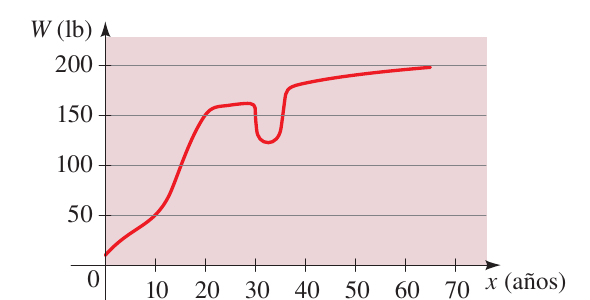
\includegraphics[width=0.68\textwidth]{fig_p03_57.png}\end{center}
\end{quote}

\begin{paso}{Paso 1 --- Localizar el único cambio de sentido}
\textbf{Qué hago:} recorro la gráfica de izquierda a derecha buscando dónde deja de subir.

\textbf{¿De dónde sale?} De la figura: el peso sube de forma continua desde $x=0$ hasta cerca de $x=30$, cae bruscamente hasta un valle cerca de $x=32$, y desde ahí vuelve a subir hasta el final de la gráfica, en torno a $x=68$.

\textbf{¿Por qué?} $W$ es creciente donde la gráfica sube y decreciente donde baja; el único tramo que baja es la caída brusca.
\[
\text{Creciente en } (0,30) \text{ y } (32,68); \qquad \text{decreciente en } (30,32).
\]
\end{paso}

\begin{paso}{Paso 2 --- Interpretar la caída de los 30 años}
\textbf{Qué hago:} traduzco a palabras el tramo decreciente hallado en el paso 1.

\textbf{¿De dónde sale?} De la gráfica: entre los $30$ y los $32$ años el peso cae de unos $160$ lb a unos $125$ lb, y luego se recupera con rapidez.

\textbf{¿Por qué?} La gráfica describe el peso en el tiempo; una caída brusca y aislada corresponde a una pérdida rápida de peso, por ejemplo una dieta o una enfermedad, seguida de la recuperación.
\end{paso}

\begin{paso}{Paso 3 --- Cambio neto de 10 a 20 años}
\textbf{Qué hago:} aplico $W(20)-W(10)$ con las alturas leídas en la cuadrícula.

\textbf{¿De dónde sale?} De la gráfica: $W(10)\approx 50$ lb y $W(20)\approx 150$ lb.

\textbf{¿Por qué?} El cambio neto es la diferencia entre el valor final y el inicial de la función.
\[
W(20)-W(10)\approx 150-50=100\ \text{lb}.
\]
\end{paso}

\begin{resp}
\emph{a}) Creciente en $(0,30)$ y $(32,68)$; decreciente en $(30,32)$. \quad
\emph{b}) Alrededor de los 30 años la persona perdió peso de golpe (una dieta o una enfermedad) y después lo recuperó. \quad
\emph{c}) Cambio neto $\approx 100$ lb (aumentó unas $100$ libras entre los 10 y los 20 años).
\end{resp}

\end{document}
